\documentclass{beamer}
\usetheme{Berlin}
\usecolortheme{beaver}
\usepackage{graphicx}
\usepackage[export]{adjustbox}
\usepackage{tikz}
\usetikzlibrary{arrows}

\title{Baseband data transmission}
\subtitle{Transmission systems, line codes and power spectra, filtering}
\author[Riccardo \and Eren]{Riccardo~Miccini\inst{1} \and Eren~Can~\inst{1}}
\institute[DTU]
{
	\inst{1}
	Technical University of Denmark\\
	Digital Communication
}
\date{\today}
\subject{Digital Communication}

\tikzstyle{int}=[draw, fill=blue!20]
\tikzstyle{every node}=[font=\tiny]

\begin{document}


	\frame{\titlepage}

	\begin{frame}
		\frametitle{Baseband transmission systems}
%		\begin{tikzpicture}[auto,>=latex']
%			\node [int] (a) {ADC};
%			\node (begin) [left of=a,node distance=1cm, coordinate] {a};
%			\node [int] (b) [right of=a] {Line coding};
%			\node [int] (c) [right of=b] {Pulse shaping};
%			\node [int] (d) [right of=c] {Channel};
%			\node [int] (e) [right of=d] {Receiver filter};
%			\node [int] (f) [right of=e] {Thresholder};
%			\node [int] (g) [right of=f] {DAC};
%			\node [coordinate] (end) [right of=g, node distance=1cm]{};
%			\path[->] (begin) edge node {Source} (a);
%			\path[->] (a) edge node {} (b);
%			\path[->] (b) edge node {} (c);
%			\draw[->] (c) edge node {} (d);
%			\draw[->] (d) edge node {} (e);
%			\draw[->] (e) edge node {} (f);
%			\draw[->] (f) edge node {} (g);
%			\draw[->] (g) edge node {} (end);
%		\end{tikzpicture}
		\begin{figure}
			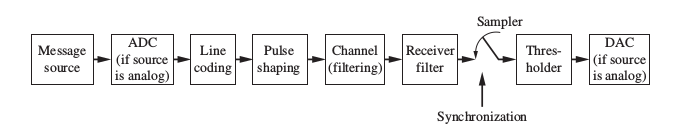
\includegraphics[width=\textwidth,keepaspectratio,center]{block_dia.png}
		\end{figure}
		\begin{description}
			\item [ADC] sampling, quantization $ \rightarrow f_s > 2W$
			\item [Line coding] generates signal according to data format
			\item [Pulse shaping, Receiver filter] optimizes signal for channel transmission
			\item [Synchronization, Thresholder] samples signal at correct time, obtain bit/symbol value
		\end{description}
	\end{frame}

	\begin{frame}
		\frametitle{Line codes (explanation)}
		\begin{itemize}
			\item NRZ - Nonreturn-to-zero
			\begin{description}
				\item [NRZ change] 1 = $V_DD$; 0 = $-V_DD$
				\item [NRZ mark] 1 = level change;  0 = no change
			\end{description}
			\item RZ - Return-to-zero
			\begin{description}
				\item [Unipolar RZ] 1 = half-width pulse, 0 = no pulse
				\item [Polar RZ] 1 = positive RZ pulse, 0 = negative RZ pulse
				\item [Bipolar RZ] 1 = alternating RZ pulse, 0 = no pulse
			\end{description}
			\item Other
			\begin{description}
				\item [Plit phase] 1 = NRZ pulse with 0-phase, 0 = NRZ pulse with $\pi$-phase
			\end{description}
		\end{itemize}
	\end{frame}

	\begin{frame}
		\frametitle{Line codes (waveforms)}
		\begin{figure}
			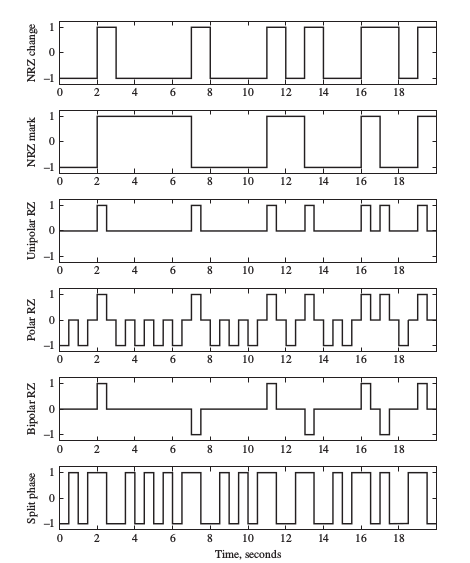
\includegraphics[width=\textwidth,height= 6.5cm,keepaspectratio,center]{line_codes.png}
		\end{figure}
	\end{frame}

	\begin{frame}
		\frametitle{Line codes (considerations)}
		\begin{itemize}
			\item Self-synchronization
			\item Channel bandwidth, frequency response
			\item Transparency
			\item Error probability and detection
		\end{itemize}
	\end{frame}

	\begin{frame}
		\frametitle{Line codes (power spectra)}
		\begin{figure}
			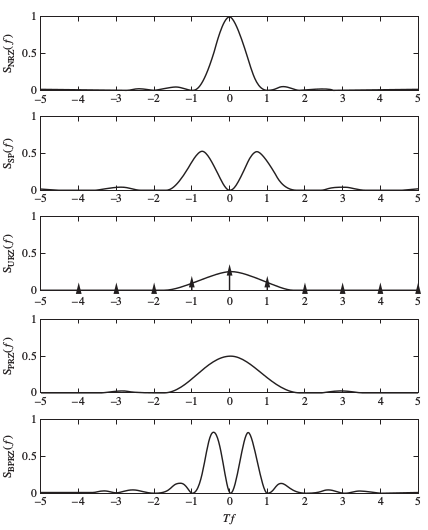
\includegraphics[width=\textwidth,height= 6.5cm,keepaspectratio,center]{lc_spectra.png}
		\end{figure}
	\end{frame}

	\begin{frame}
		\frametitle{ISI - Intersymbol interference}
		\begin{itemize}
			\item Caused by insufficient channel BW
			\item Shallower pulses, symbol bleeding
			\item Solutions:
			\begin{itemize}
				\item Proper pulse shaping and receiver filter
				\item Equalization
			\end{itemize}
		\end{itemize}
	\end{frame}

\end{document}
